\documentclass[a4 paper]{article}
% Set target color model to RGB
\usepackage[inner=2.0cm,outer=2.0cm,top=2.5cm,bottom=2.5cm]{geometry}
\usepackage{setspace}
\usepackage[rgb]{xcolor}
\usepackage{verbatim}
\usepackage{subcaption}
\usepackage{amsgen,amsmath,amstext,amsbsy,amsopn,tikz,amssymb,tkz-linknodes}
\usepackage{fancyhdr}
\usepackage[colorlinks=true, urlcolor=blue,  linkcolor=blue, citecolor=blue]{hyperref}
\usepackage[colorinlistoftodos]{todonotes}
\usepackage{rotating}
%\usetikzlibrary{through,backgrounds}
\hypersetup{%
pdfauthor={Ashudeep Singh},%
pdftitle={Assignment 3},%
pdfkeywords={Tikz,latex,bootstrap,uncertaintes},%
pdfcreator={PDFLaTeX},%
pdfproducer={PDFLaTeX},%
}
%\usetikzlibrary{shadows}
% \usepackage[francais]{babel}
\usepackage{booktabs}
\newcommand{\ra}[1]{\renewcommand{\arraystretch}{#1}}

\newtheorem{thm}{Theorem}[section]
\newtheorem{prop}[thm]{Proposition}
\newtheorem{lem}[thm]{Lemma}
\newtheorem{cor}[thm]{Corollary}
\newtheorem{defn}[thm]{Definition}
\newtheorem{rem}[thm]{Remark}
\numberwithin{equation}{section}

\newcommand{\homework}[6]{
   \pagestyle{myheadings}
   \thispagestyle{plain}
   \newpage
   \setcounter{page}{1}
   \noindent
   \begin{center}
   \framebox{
      \vbox{\vspace{2mm}
    \hbox to 6.28in { {\bf COMP 3005:~Database Management Systems \hfill {\small (#2)}} }
       \vspace{6mm}
       \hbox to 6.28in { {\Large \hfill #1  \hfill} }
       \vspace{6mm}
       \hbox to 6.28in { {\it Instructor: {\rm #3} \hfill Name: {\rm #5}, ID: {\rm #6}} }
       %\hbox to 6.28in { {\it TA: #4  \hfill #6}}
      \vspace{2mm}}
   }
   \end{center}
   \markboth{#5 -- #1}{#5 -- #1}
   \vspace*{4mm}
}

\newcommand{\problem}[2]{~\\\fbox{\textbf{Q #1}}\hfill (#2 points)\newline\newline}
\newcommand{\subproblem}[1]{~\newline\textbf{(#1)}}
\newcommand{\D}{\mathcal{D}}
\newcommand{\Hy}{\mathcal{H}}
\newcommand{\VS}{\textrm{VS}}
\newcommand{\solution}{~\newline\textbf{\textit{(Solution)}} }

\newcommand{\bbF}{\mathbb{F}}
\newcommand{\bbX}{\mathbb{X}}
\newcommand{\bI}{\mathbf{I}}
\newcommand{\bX}{\mathbf{X}}
\newcommand{\bY}{\mathbf{Y}}
\newcommand{\bepsilon}{\boldsymbol{\epsilon}}
\newcommand{\balpha}{\boldsymbol{\alpha}}
\newcommand{\bbeta}{\boldsymbol{\beta}}
\newcommand{\0}{\mathbf{0}}



\begin{document}
\homework{Assignment \#3}{Due: Friday November 5, 2021 (11:59 PM)}{Ahmed El-Roby}{}{}{}
\textbf{Instructions}: Read all the instructions below carefully before you start working on the assignment, and before you make a submission.
\begin{itemize}
    \item The accepted format for your submission is pdf only.
    \item If you use the tex file, make sure you edit line 28 to add your name and ID. Only write your solution and do not change anything else in the tex file. If you do, you will be penalized.
    \item No late submissions are allowed.
\end{itemize}



\problem{1:}{11}
Design a database for a national family medicine practice with a set of patients and a set of medical doctors. The database should capture the relationship between doctors and patients, where a patient can possibly have a family doctor, or multiple doctors. The database should also store the patients tests. The tests can be ordered by one or more doctors, but this is not mandatory since a test can be ordered by a nurse practitioner (no need to model nurses). The database should keep track of the dates of the tests as well as their results. Draw an ER-diagram for your design. Feel free to include any attributes you find relevant to this database. Underline the primary key in the entity sets.

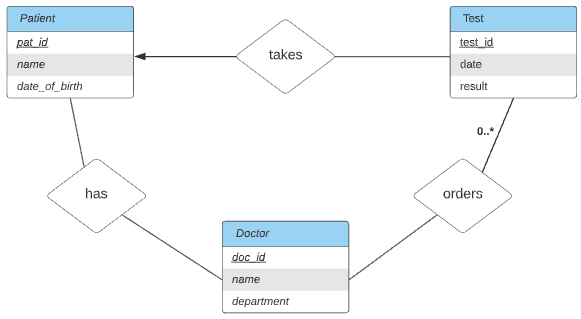
\includegraphics[width=\textwidth]{er1.png}

Assumptions: 
It is possible for patients to not have a doctor and a doctor to not have any patients. Patients can take many tests, a test is only done on one patient. Patients can have many doctors and doctors can have many patients.
Doctors can order many tests and tests can be done by nurse practitioners or doctors. A nurse practitioner does not count as a doctor.
So, a test can be performed by 0 to many doctors, 0 being it is done by a nurse practitioner.

\problem{2:}{6}
Reduce your ER-diagram to relations. Underline primary keys.

patient(\underline{pat\_id}, name, date\_of\_birth)

doctor(\underline{doc\_id}, name, department)

test(\underline{test\_id}, date, result)

takes(\underline{pat\_id}, test\_id)

has(\underline{pat\_id}, doc\_id)

orders(\underline{doc\_id}, test\_id)

\problem{3:}{5}
If any test must be ordered by a doctor, what needs to be changed in your answer to Q1? Either draw a new ER-diagram, or describe the changes. How will the reduced relations change?

If any test must be ordered by a doctor then the cardinality changes. Since a test cannot be ordered by a nurse practitioner now and must be ordered by a doctor.
A test must have 1 or more doctors.

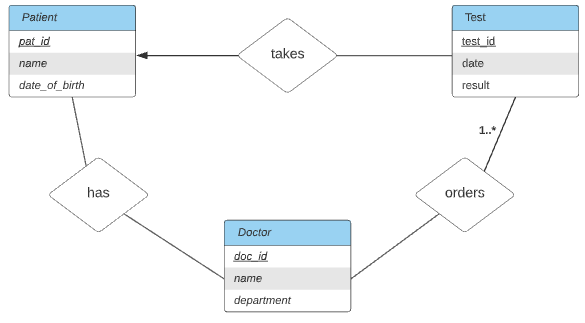
\includegraphics[width=\textwidth]{er3.png}

\problem{4:}{14}
Consider the following ER diagram for a database design for a car insurance company:

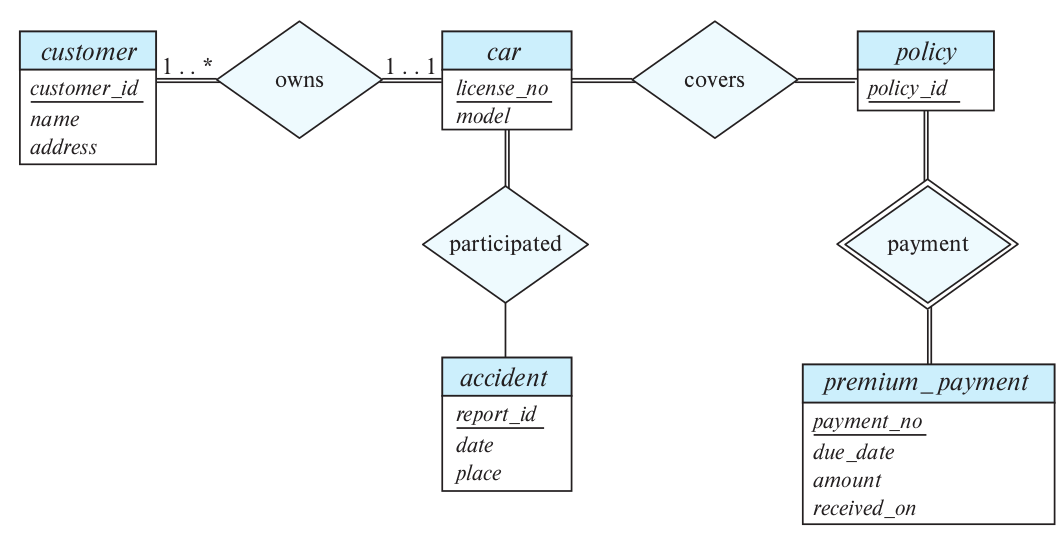
\includegraphics[width=\textwidth]{er2.png}

\noindent Construct the relation schemas for this ER diagram.

customer(\underline{customer\_id}, name, address)

owns(\underline{customer\_id}, license\_no)

car(\underline{license\_no}, model)

covers(\underline{license\_no}, policy\_id)

policy(\underline{policy\_id})

participated(\underline{report\_id}, license\_no)

accident(\underline{report\_id}, date, place)

payment(\underline{policy\_id}, \underline{payment\_no}, due\_date, amount, received\_on)

premium\_payment(\underline{policy\_id}, \underline{payment\_no}, due\_date, amount, received\_on)


\end{document}


\end{document}

